\justifying

The Sun is our nearest astrophysical object, which serves as a natural laboratory for various branches of Physics - atomic physics, spectroscopy, turbulence, magneto-hydrodynamics, stellar evolution, dynamo and magnetism and plays a key role in space and terrestrial weather. The Sun is also the primary source of light and energy on earth. So it is only natural that we try to understand the different physical processes involved in the energectics of the Sun, which indirectly affects life on Earth. In this chapter I briefly introduce the Sun and various layers of its atmosphere. At the end we provide a motivation for the thesis.

The Sun is a G2V star, with surface luminosity $3.86~\times~10^{26}$ W and an effective temperature of $\sim 5780~K$. The Sun is mostly made out of Hydrogen(92.1\%) and Helium(7.8\%) along with negligible quantities of heavier elements C, N, O, Mg, Si, Ne and Fe. The study of the Sun can be mainly divided into three components: the Solar interior, the Solar atmosphere and the Heliosphere.

%%%%%%%%%%%%%%%%%%%%%%%%%%%%%%%%%%%%%%%%%%%%%%%%%%%%%%%
\section{The solar interior}\label{solar_int}
%%%%%%%%%%%%%%%%%%%%%%%%%%%%%%%%%%%%%%%%%%%%%%%%%%%%%%%

In the innermost zone of the star the Sun has a temperature of about 15 MK and a density of $1.6~\times~10^{5}~km.m^{-3}$ that fuses Hydrogen into Helium mainly by p-p cycle \citep{bethe38} and to some extent by CNO cycle \citep{bethe39}. 

%% ############# %%
\begin{figure}[h!]
    \centering
    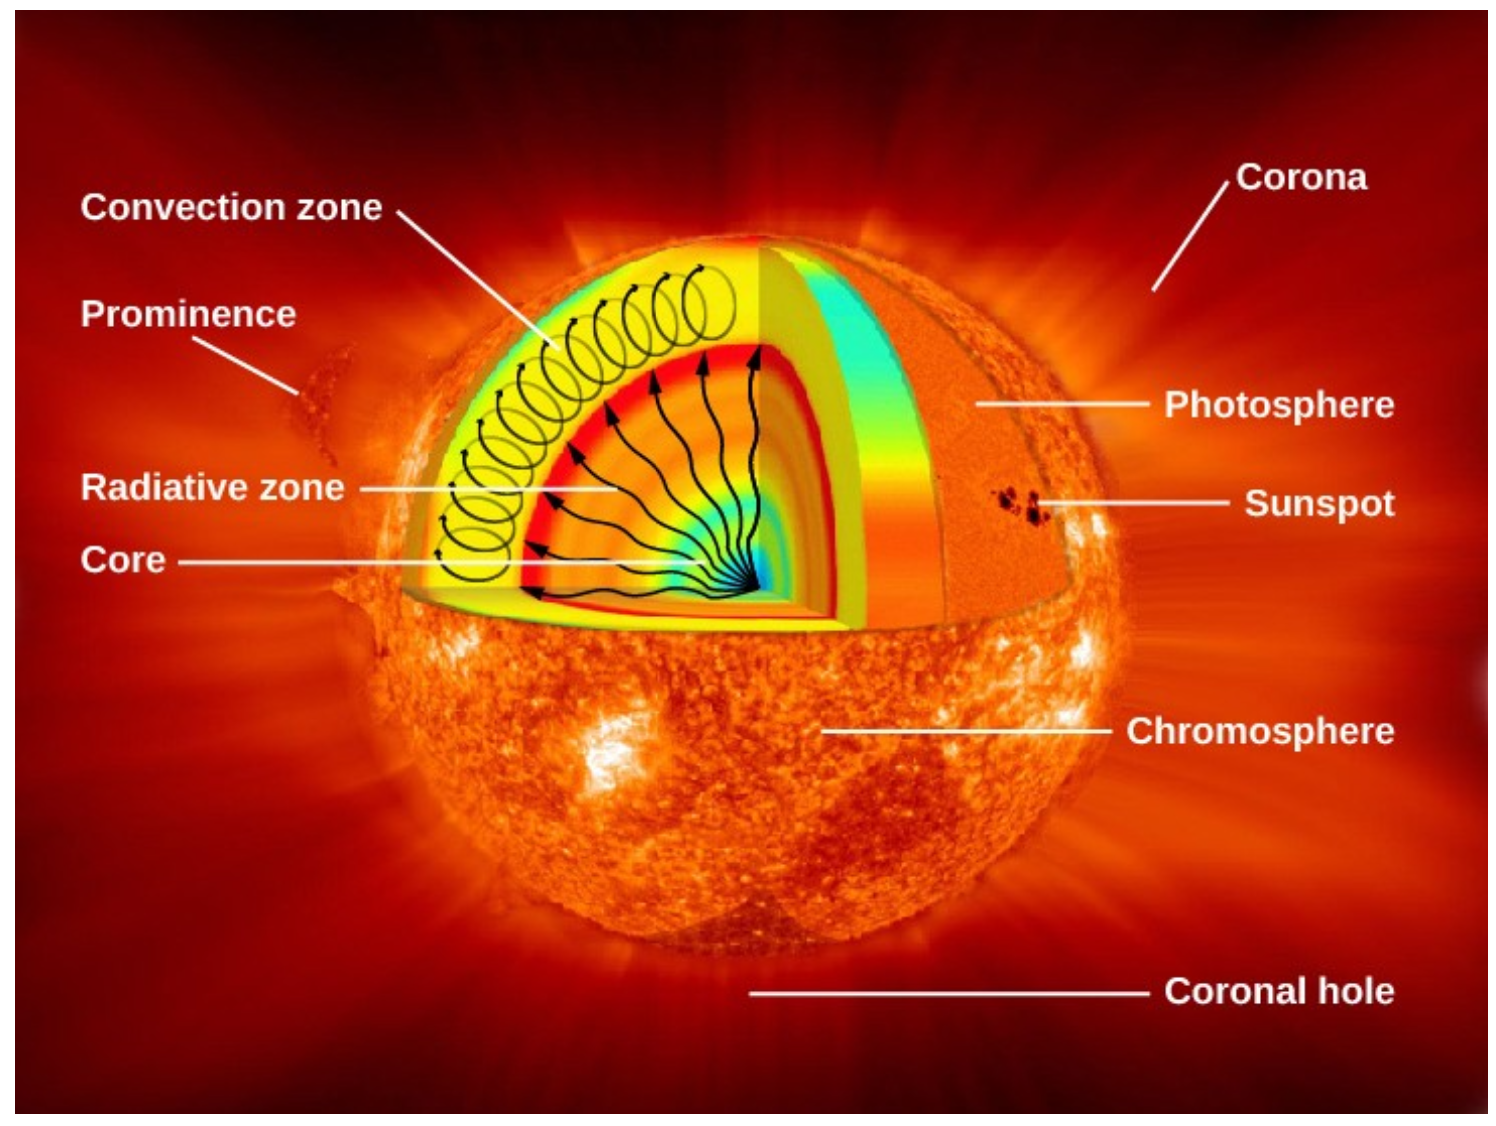
\includegraphics[width = 0.8\linewidth]{Figures/solar_int.png}
    \caption{A schematic depiction of the different layers of the Sun. The figure also shows some of the most prominent magnetic structures on the Sun e.g sunspot, prominence, coronal hole. Credit : NASA/Goddard.}
    \label{fig_solar_int}
\end{figure}
%% ############# %%

Fig.~\ref{fig_solar_int} shows a schematic diagram of various layers of the Sun. Beyond the core we have the optically thick radiative zone, where the Hydrogen and Helium are completely ionized. The high energy $\gamma$-ray photons generated in the core, have very small mean free path in this region, as they collide numerous times eventually thermalizing becoming visible photon. Beyond the radiative zone the degree of ionization of Hydrogen and Helium changes drastically giving rise to a sharp temperature gradient. This is the convective zone where the energy from the inner layers of the Sun is transported adiabetically to the surface of the Sun. In between the radiative and the convective zone, there is a thin layer, roughly at $\sim~0.7~R_{\odot}$ known as the tacholine, which is believed to play a major role in generating Sun's magnetic field via the Dynamo process \citep{corbard01}. 

The core and the radiative zone of the Sun rotates as a solid body, whereas the convective zone rotates differentially. The rotation period varies from $\sim~25~days$ to $\sim~35~days$ from the equator to the pole.

%%%%%%%%%%%%%%%%%%%%%%%%%%%%%%%%%%%%%%%%%%%%%%%%%%%%%%%
\section{The solar atmosphere}\label{solar_atmos}
%%%%%%%%%%%%%%%%%%%%%%%%%%%%%%%%%%%%%%%%%%%%%%%%%%%%%%%

The layers outside the convection zone together, form the solar atmosphere - the Photosphere, which is also known as the Sun's surface, the Chromosphere, the transition region and the Corona. While we can define geometrical height or depths to define these layers, it is much more useful to define them using the local optical depths of various spectral lines, which are directly used to observe the layers. This also gives us a idea about which spectral features originate mainly from which portions of the solar atmosphere. Fig.~\ref{fig_solar_atm} shows the variation of temperature and number density across various layers of the Solar atmosphere \sr{Ref. here}.

%% ############# %%
\begin{figure}[h!]
    \centering
    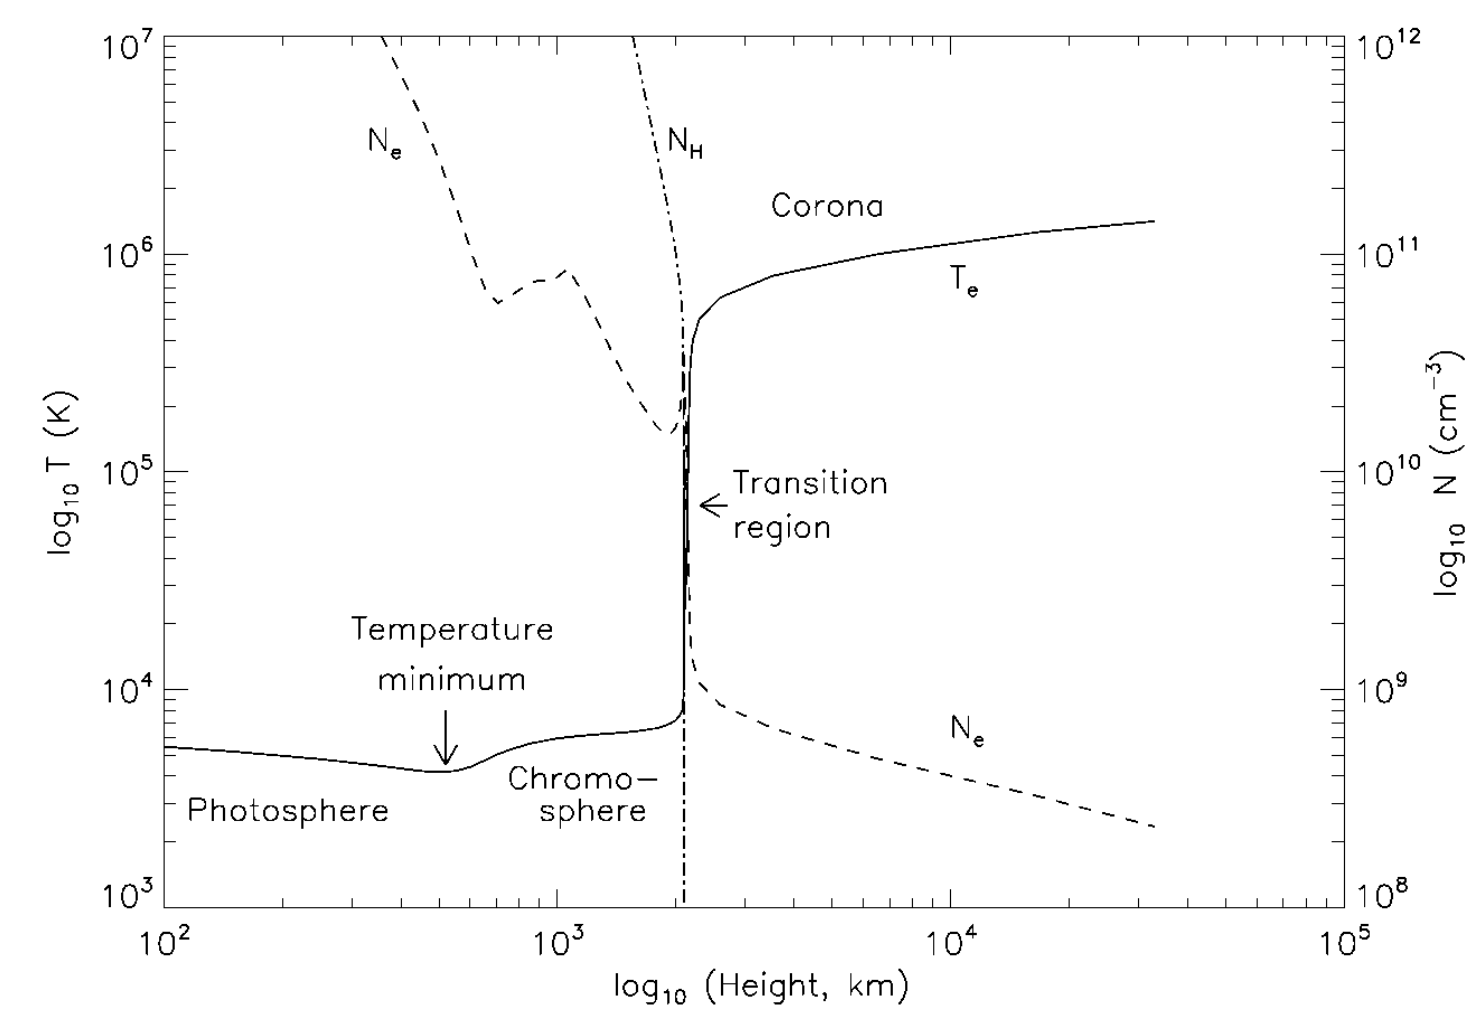
\includegraphics[width = 0.8\linewidth]{Figures/solar_atm.png}
    \caption{The variation of electron temperature (solid line) and electron density ($\mamthrm{N_{e}}$, dashed line) and density of neutral hydrogen atoms ($\mathrm{N_{H}}$, dotted- dashed line) in the solar atmosphere as derived based on the 1-D model calculations by \sr{Ref. here}.}
    \label{fig_solar_atm}
\end{figure}
%% ############# %%

%%%%%%%%%%%%%%%%%%%%%%%%%%%%%%%%%%%%%%%%%%%%%%%%%%%%%%%
\subsection{The Photosphere}\label{photosphere}
%%%%%%%%%%%%%%%%%%%%%%%%%%%%%%%%%%%%%%%%%%%%%%%%%%%%%%%

The Photosphere is defined to be the layer where $\tau_{\lambda~\sim~5000}~=~1$. This is in the green part of the visible spectrum and the Sun is opaque in visible beyond this layer, hence it is called to be the surface of the Sun. This layer is 400-600 km deep and has an effective temperature of 5780 K. The magnetic filed lines arising from the tacholine penetrate the Photosphere and creates a `carpet' over the whole region \citep{priest14}. As mentioned earlier, this is the Solar surface known as the `Quite Sun'(QS). This region exhibits an average magnetic flux density of \textbf{10 -- 50~G}. The QS surface is covered with cells of roughly four size- granule, meso granules, super granules and giant cells. Some regions exhibit much stronger magnetic flux density often associated with highly twisted magnetic field structures. These magnetic features are manifested as sunspots, spicules, bright points etc. 

As the density changes drastically at the Photosphere compared to the convective zone, the thermalized photons from Sun's core start free streaming again, as the mean free path also increases drastically and as a result perturbs the thermal equilibrium (TE from hereon). So, we have to define the thermodynamic quantities of the Photosphere in Local Thermal Equilibrium (LTE from hereon). As we move away from the Photosphere, because the density keeps on decreasing steadily, the LTE conditions also start deviating similarly \citep{philips08}.

%%%%%%%%%%%%%%%%%%%%%%%%%%%%%%%%%%%%%%%%%%%%%%%%%%%%%%%
\subsection{The Chromosphere}\label{chromosphere}
%%%%%%%%%%%%%%%%%%%%%%%%%%%%%%%%%%%%%%%%%%%%%%%%%%%%%%%

The Chromosphere is a highly non-uniform dynamic layer with a thickness of 1500~--~3000~km, with increasing temperature (upto $10^{4}$ K) and decreasing number density. As seen in the fig. \ref{fig_solar_atm}, the temperature of the Chromosphere saturates before the dramatic rise in the transition region. This saturation is attributed to a steady deposition of acoustic energy by creation of shock waves \citep{carlsson07}. The Chromosphere also exhibits a sharp gradient in the plasma $\beta$ factor, non-LTE conditions, dominance of wave motions \sr{Ref. here}. 

%%%%%%%%%%%%%%%%
\begin{figure}[ht!]
    \centering
    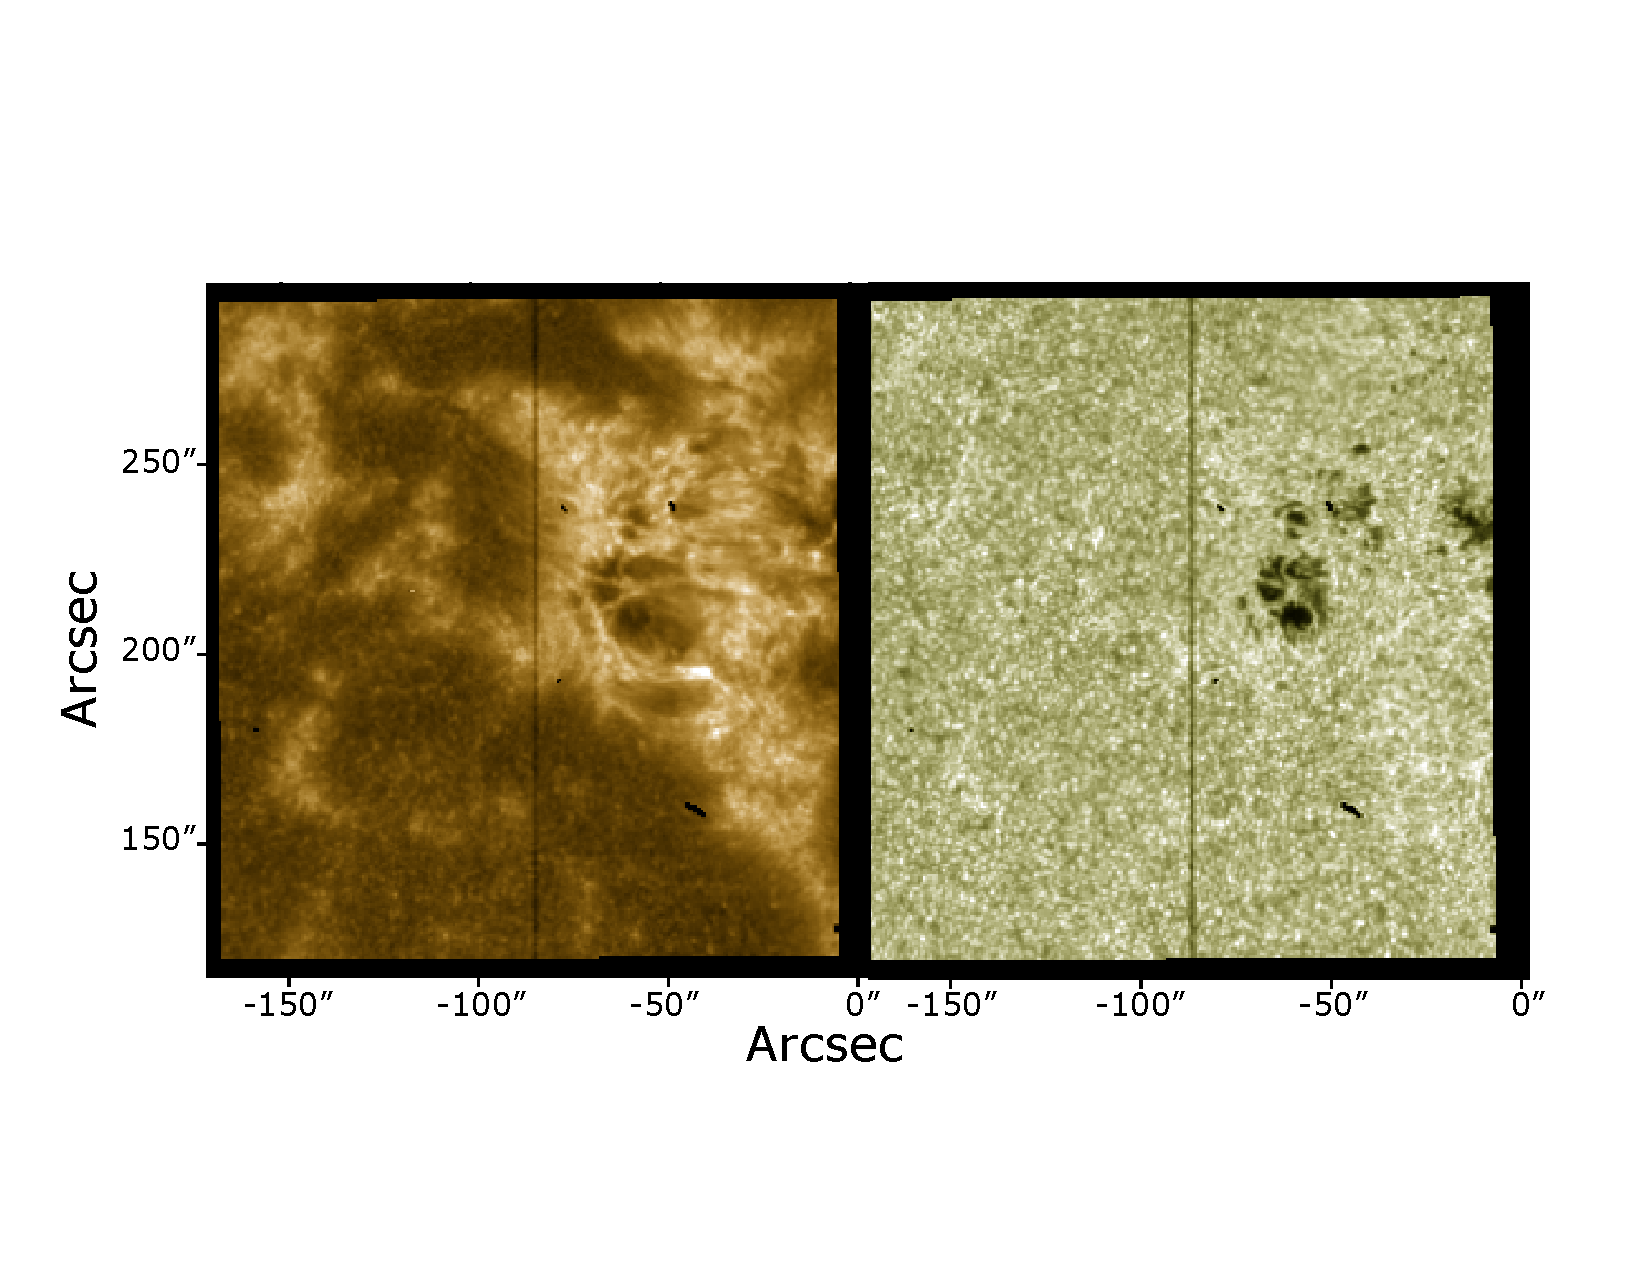
\includegraphics[trim={1cm 3cm 2cm 5cm},clip,width=0.8\textwidth]{Figures/sji_images.pdf}
    \caption{IRIS SJI Slit-jaw images of NOAA AR 13521 on Dec 21st, 2023 in \ion{Mg}{2} 2796 {\AA}~(left panel) showing the upper Chromosphere. The right panel shows the same active region in 2832 {\AA}~continuum corresponding to upper photosphere.}
    \label{fig:sji_features}
\end{figure}
%%%%%%%%%%%%%%%%

In fig.~\ref{fig:sji_features} we show the NOAA AR 13521 in IRIS SJI 2796 {\AA} (left panel) and 2832 {\AA} (right panel). The dark sunspots and plage regions surrounding it are clearly visible in the 2832 {\AA} wavelength window. In the 2796 {\AA} window we see the plage along with light bridges more clearly. 

%%%%%%%%%%%%%%%%%%%%%%%%%%%%%%%%%%%%%%%%%%%%%%%%%%%%%%%%%%%%%%%%%%%
\subsection{The Transition Region}\label{transition-region}
%%%%%%%%%%%%%%%%%%%%%%%%%%%%%%%%%%%%%%%%%%%%%%%%%%%%%%%%%%%%%%%%%%%

The transition region above the Chromosphere is a thin, dynamic layer where we witness a dramatic increase in temperature by two orders of magnitude along with a similar decrease in electron density by nearly 5-6 orders of magnitude which is demonstrated in fig. \ref{fig_solar_atm}. In general the this layer is roughly $\sim$ 100 km in thickness, but that can change depending on various dynamic conditions of Chromosphere($\sim~10^{4}~K$) below, or Corona($\sim~10^{6}~K$) on top. The transition region is generally characterized by the steep change in the temperature, pressure gradients, drastic change in local optical depth and competition between gas pressure and magnetic pressure. The transition region also manifests the ARs as various magnetic features such as small scale brightening, jets, spicules, fibrils etc. 

%%%%%%%%%%%%%%%%%%%%%%%%%%%%%%%%%%%%%%%%%%%%%%%%%%%%%%%%%%%%%%%%%%%
\subsection{The Corona}\label{corona}
%%%%%%%%%%%%%%%%%%%%%%%%%%%%%%%%%%%%%%%%%%%%%%%%%%%%%%%%%%%%%%%%%%%

The outermost layer of the Solar atmosphere is the Corona. The Corona is only visible in naked eyes during the total solar eclipse or via Coronagraphs. It maintains a steady temperature of 1-2 Mk during ambient conditions, but can rise upto tens of MK during solar flares. The coronal continuum spectrum is produced due to Thompson scattering of photons from photosphere off coronal electrons. Corona also emits in various emission lines, e.g. Mg, Fe, Si, S, Ca, O etc. across a wide band of electromagnetic spectrum ranging from X-ray to visible wavelengths. 

Similar to the other layers, the corona exhibits a variety of structures such as ARs, coronal holes, bright points, filaments, flares. The flare arcades are most prominently visible in the Corona. So, most of our existing studies over the last decade has focused on the coronal features of the flares. In fig.~\ref{fig:sji_features} we show one of the most well known and well studied solar eruptions from Aug 31st, 2012. A giant prominence erupted from the south east limb. The erupted prominence material was visible in all AIA channels from 304 \AA~(Chromospheric He II, see fig.~\ref{fig:aia-feature} \textbf{panel (a)}) across all six Coronal channels (\textbf{panel (b){--}(g)}). The sun spots were also clearly visible in HMI magnetogram and continuum (see fig.~\ref{fig:aia-feature} \textbf{panel (h)}). In \textbf{panel (i)} we show the co-aligned AIA 304 \AA, 131 \AA and HMI magnetogram image. The sunspots lie at the base of the erupted prominence, accompanied by the hot thermal plasma associated with the accompanying flare. The novelty of such observation lies in the clear spatial connection across various layers of the sun, connected via energy and momentum transported from one layer to the other. 

%%%%%%%%%%%%%
\begin{figure}
    \centering
    \includegraphics[width=\textwidth]{Figures/aia_features.pdf}
    \caption{Image of the prominence eruption and associated flare from NOAA AR 11562 on Aug 31st, 2012$\sim$19:50 UT. The prominence is visible in all of the AIA channels. We see the coronal holes in AIA 335 \AA~\textbf{(panel c)}. The flare loops of the associated event is visible in AIA 94 \AA~\textbf{(panel e)} and AIA 131 \AA~\textbf{(panel f)}. The sunspots are visible in HMI continuum \textbf{panel (h)}. We show a co aligned map of AIA 304 \AA, HMI magnetogram and AIA 131 \AA~in \textbf{panel (i)}. The spatial association of the sunspots with the hot flareloop plasma and the prominence eruption is clearly demostrated here. }
    \label{fig:aia-feature}
\end{figure}
%%%%%%%%%%%%%




%%%%%%%%%%%%%%%%%%%%%%%%%%%%%%%%%%%%%%%%%%%%
\section{Solar Flares}\label{sol_flr}
%%%%%%%%%%%%%%%%%%%%%%%%%%%%%%%%%%%%%%%%%%%%

Solar flares are the most powerful magnetic events in the solar system. They are described as a sudden increase in brightness in localized areas on Sun. Within tens of minutes, they can release over $10^{32}$ erg of energy, which is emitted across the entire electromagnetic spectrum from radio to gamma rays. They can also launch high energetic particles into the interplanetary medium. Most of the flares occur in magnetic active regions, and the amount of flare energy released is comparable to the free energy stored in the magnetic system. The term "flare" is generally used explicitly for the entire magnetically-driven event's electromagnetic radiation, as it is the most significant fraction of the total energy liberated. The total energy released varies from event to event. It is also known that larger events occur much less frequently than smaller events.

%% ##################################################### %%
\subsection{Brief history of flare observation}\label{sol_flr_1}
%% ##################################################### %%

In September 1, 1859, R.C. Carrington and R. Hodgson observed the first flare in the continuum of white light\citep{carrington1859,hodgson1859}. The localized brightening on the Sun have remained an enigma ever since. We have been observing the local flaring events across all wavelengths from both ground and space based observatories.  Shortly after the observation by Carrington and Hodgson, people started studying the Sun extensively in the H$\alpha$ line which is formed in the Chromosphere, and the reports of flaring events became more and more frequent and progressively more and more complex. No two events were similar, as there were variations observed in source of size, ejections of plasma along with shock waves driving into the interplanetary space. Advances of radio technology during the second world war ensured detection of presence of non-thermal electrons in the solar corona, during military radar operations \citep{hey46}. Around the same time S.E. Forbrush noticed ground level cosmic ray enhancement during major solar flares. These discoveries eluded that the flaring events do not only involve the thermal plasma, but is somehow connects with high energy particles and involves the corona. in the 1950s we started observing the Sun in hard X-rays ($\ge~10~keV$) with rockets and balloons. \cite{peterson59} discovered the first hard X-ray emission during a flare in 1958. Later on, it was deduced from the observations of the enhancements observed in radio and hard X-rays that, the the ejected energetic particles may contain a substantial fraction of the initial energy released \citep{brown71}. The hard X-ray is created by the bremsstrahlung of the electrons colliding into dense material, resulting in a power-law energy distribution. The broadband radio emission from 1 to 100 GHz is created from gyrosynchrotron emission. Finally, observations in EUV and soft X-ray($\le$~10~keV) have shown that the energy released form the flare heats the plasma contained in the coronal loops to temperatures beyond 30 MK. 

%% ################################################################# %%
\subsection{Neupert effect}\label{npt_eff}
%% ################################################################# %%

\cite{neupert68} observed a curious correlation that, the soft X-ray flux during the rise phase of the flare is proportional to the time integral of the centimeter radio flux since the start of the flare. The centimeter radio flux is emitted by relativistic electrons. So, later on the same correlation was found between the hard X-ray flux and soft X-ray flux and can be expressed as,

%%%%%%%%%%%%%%%%%%%%%%%%%%%%%%%%
\begin{equation}\label{npt_eff_eq}
    F_{SXR}(t)~\propto~\int_{t_{0}}^{t}~F_{HXR}(t')~dt'
\end{equation}
%%%%%%%%%%%%%%%%%%%%%%%%%%%%%%%%

This empirical relation is known as the ``Neupert effect''. \cite{neupert68} had already suggested that this may be due to a causal relationship between the thermal plasma and the energetic electrons. The logical explanation is: the soft X-ray mainly originates from a thermal plasma heated by the energy of the flaring event deposited by the flare accelerated electrons. It is important to mention that we know now, Eqn.\ref{npt_eff_eq} is only valid if cooling by conduction of radiation is negligible.

%% ################################################################# %%
\subsection{``Standard'' model of solar flare}\label{sol_flr_std_mod}
%% ################################################################# %%

There were several observations like Neupert effect, which would help us to constrain several phenomenon observed in the flares:

%%%%%%%%%%%%%%%%%%%%%%%%%%%%%%%%%%
\begin{figure}[h!]
    \centering
    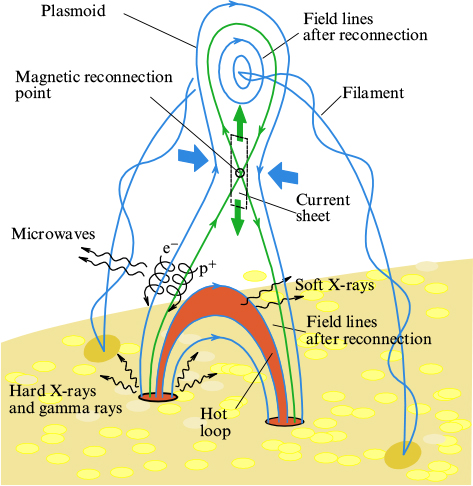
\includegraphics[width=0.5\linewidth]{Figures/phu_63_8_818_f2.jpg}
    \caption{A schematic diagram of the standard model of solar flare (adapted from \cite{lysenko20}).}
\end{figure}
%%%%%%%%%%%%%%%%%%%%%%%%%%%%%%%%%%

%%%%%%%%%%%%%%%%%
\begin{enumerate}
    \item The magnetic reconnetion happens in corona, releasing the magnetic free energy. Electrons and energetic particles from the reconnetion site are accelerated along the realigned magnetic field lines. The accelerated particles that escape along the open field lines towards the earth gives rise to the particle events seen from earth.
    \item The accelerated particles move along the field lines downwards along the magnetic field lines, giving rise to the microwave observations seen from flares via gyro magnetic radiation.
    \item The accelerated particles hit the Chromosphere which is considerably denser than the Corona, giving rise to Hard X-ray and gamma ray observed from the foot points. This also explains why the coronal hard X-ray source is considerably softer than the foot points. The energetic particles deposit their energy into the local Chromosphere, as they go through series of collision and eventually thermalize.
    \item  As the plasma thermalizes, it starts emitting in thermal bremsstrahlung giving rise to the soft X-ray observed. Also, as the energy is deposited into the Chromosphere from the accelerated particles, it heats the local Chromosphere environment it gradually increases the local pressure. 
    \item As the pressure grows, when the pressure gradient builds up enough the local plasma starts expanding upwards(essentially due to buoyancy) and slowly fills up the coronal loops with soft X-ray emitting plasma. This phenomenon is known as "Chromospheric evaporation". This was directly observed later on, in blue-shifted lines of hot material.
    \item This whole scenario explains the Neupert effect. As the energy form the accelerated particles is converted into the soft X-ray emitting plasma, and it builds up over time. That explains the soft X-ray being proportional to the time integral of the hard X-ray flux.
\end{enumerate}
%%%%%%%%%%%%%%%%%

This whole scenario is known as the ``Standard'' model of solar flare. While the standard model is an attempt to explain and unify various kind of differences seen from the numerous flares we observe, there are several cases where the standard model cannot explain the observations. For example, there have been observations of flares where the hard X-ray foot point do not form. It is proposed that in these cases the plasma in the coronal loops is so dense that the accelerated particle collide enough to thermalize within the flare loops before reaching the Chromosphere, defusing the energy more evenly within the loop, rather than dumping it at the base of the loops \citep{veronig02,veronig04}. Another flare which previously occurred at the same region might explain the denser coronal loops \citep{strong84,bone07}.  

%% ################################################################# %%
\subsection{The energectics of solar flares}\label{sol_flr_energ}
%% ################################################################# %%

With an experience of observing solar flares for more than 150 years, remarkably enough, we have barely started scratching the surface of the complexity involved with the solar flares. The re-configuring of magnetic structure, which almost always involves complex geometry, making almost all events unique in some sense. After that the released magnetic free energy is transported across various layers of the sun and converted into various other forms of energy. Considering how the energy is transformed the magnetic energy of the active region that is released after the reconnection into the reconnection outflow jets, the kinetic energy of escaping particles, the thermal and the kinetic energy of the Chromospheric plasma evaporating, the radiative and conductive losses. In case of the eruptive events, there is the added complexity of the kinetic and potential energy of the CMEs, the energy of the shocks and the kinetic energy of the solar energetic particles. 

In order to constrain the models of solar eruptions and various nuanced aspects of it, like magnetic reconnection, particle acceleration, heating etc. detailed quantitative characterization is absolutely necessary. There have been several studies that have tried to quantify the partition between various subsets of the energies. The questions that are particularly important are:

%%%%%%%%%%%%%%%%%%%%%%%%%%%%%%%%%%%%%%%%%%%%%
\begin{itemize}
    \item \textbf{If an active region can have enough free energy to account for the total energy released in the solar flares and/or CMEs.}
    \item \textbf{What is the energy partition between flares and CMEs.}
    \item \textbf{If the non-thermal component have enough energy to power up the thermal component.}
\end{itemize}
%%%%%%%%%%%%%%%%%%%%%%%%%%%%%%%%%%%%%%%%%%%%%

It is generally well known by now that the active region have enough magnetic free energy to power the flare and CME \citep{emslie12,ash17}. The partition of energy between the flare and associated CME is much more fuzzy. \cite{emslie12} found that the flare and CME have energies of same order of magnitude, while \cite{ash17} concluded the flare dominates the CME in-terms of the energy. However the simple question, whether the non-thermal component of the flares have enough energy is still not resolved as even the most recent studies contradict each other in the most puzzling fashion. \cite{warmuth20} discussed the contradictions arising from some of the studies\citep{stosire07,emslie12,inglis14,warmuth16a,warmuth16b,ash17}. The details of the studies can be summarized as follows:

%%%%%%%%%%%%%%%%%%%%%%%%%%%%%%%%%%%%%%%%%%%%%%%
\begin{table}[h!]
    \centering
    \hline 
    \hline
    \resizebox{\textwidth}{!}{%
    \begin{tabular}{||c|c|c|c|c|c|c||}
       Study & No. of flares & GOES class range & Thermal model & Thermal spectrum & Thermal volume & Thermal losses \\
       \cite{stosire07} (S07 from hereon) & 18 & A3-B7 & Isotherm. & RHESSI & TRACE & X \\
       \cite{emslie12} (E12 from hereon) & 38 & C5-X28 & Isotherm. & RHESSI & RHESSI & Rad. \\
       \cite{inglis14} (IC14 from hereon) & 10 & B3-B9 & Multitherm. & RHESSI+AIA & RHESSI & Rad. \\
       \cite{warmuth16a,warmuth16b} (WM16 from here on) & 24 & C3-X17 & Isotherm. & RHESSI+GOES & RHESSI & Rad.,Cond. \\
       \cite{ash17} (A17 from here on) & 188 & M1-X7 & Multitherm. & AIA & AIA & Rad. \\
       \hline
    \end{tabular}}
    \caption{The details of the studies.}
    \label{tab1}
\end{table}
%%%%%%%%%%%%%%%%%%%%%%%%%%%%%%%%%%%%%%%%%%%%%%%

The bolometric energy serves as a representation of the overall energy released during solar flares. Regardless of how energy is released in a solar flare, whether through direct plasma heating, rapid bulk flows, or non thermal particle processes—the ultimate outcome is thermalization and subsequent radiation across the electromagnetic spectrum. Given that bolometric energy encompasses the entire spectrum, it is anticipated to reflect the total energy originally released. It's important to note that this specifically pertains to the energy liberated within the flare and does not encompass the energy associated with a concurrent coronal mass ejection (CME) or filament eruption. \cite{warmuth20} used the bolometric energy released in solar flares, to compare various studies on equal footing. Here we will discuss some of the main issues \cite{warmuth20} identifies comparing these studies.

The calculated thermal energy of all studies show an excellent correlation with the {\it GOES} class. Fig.~\ref{fig:goes-therm} left panel shows the peak thermal energy as a function of peak {\it GOES} flux for all the flares from the five studies. EM12 and WM16 are consistently one order of magnitude lower than the bolometric energy. Interpolation of E12 and WM16 are about half an order of magnitude lower compared to IC14, while S07 is very consistent with the extrapolation. The energies of A17 is about an order of magnitude higher compared to other studies, and even higher than the extrapolated bolometric energy for flares of same class from \cite{kretzschmar11} and E12. There can be several reason of these differences between the studies arising.

A possible reason can be attributed to different thermal models used to model the thermal component of the flares. {\it RHESSI} usually yields a higher temperature and lower emission measure compared to {\it GOES} due to the highly multi thermal nature of the flaring plasma \citep{bataglia05,ryan14,warmuth16a}. Although the {\it GOES} temperature is higher by a factor of 1.4, it is not dependant on the flare class. Along with that, \cite{warmuth20} also investigated whether assuming a isothermal or multi thermal model introduces any differences in the thermal energy estimates. They reported no significant differences due to differences of models (refer to Fig. 2 and the corresponding discussion in \cite{warmuth20}).

%%%%%%%%%%%%%%%%%%%%%%%%%%%%%%%%%%%%%%%%%%%%%%%
\begin{figure}[ht!]
    \centering
    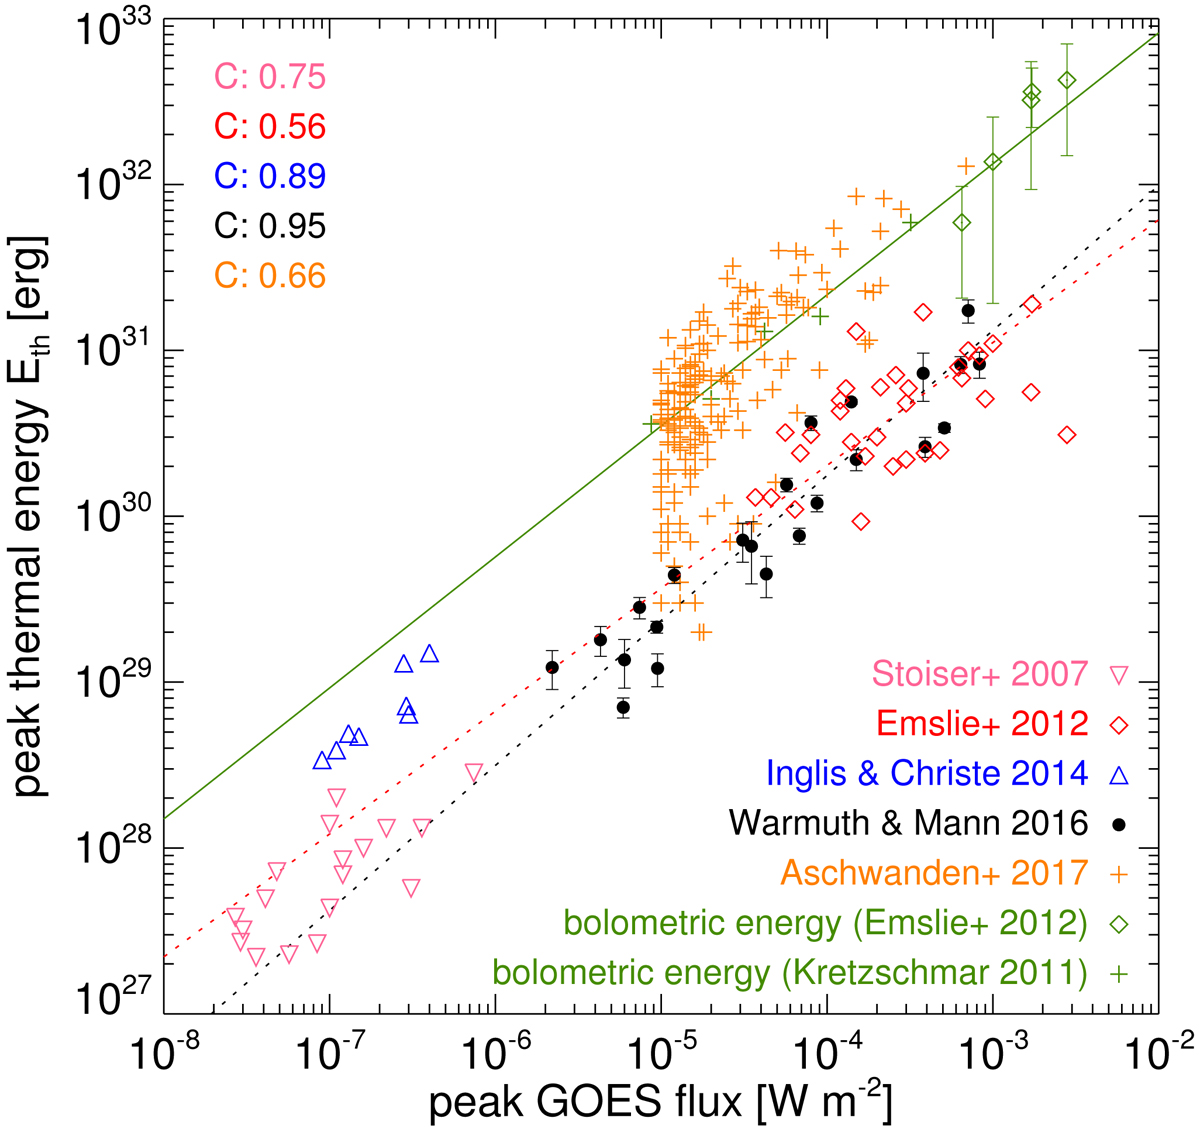
\includegraphics[width=0.45\textwidth,trim={0cm 0cm 0cm 0.02cm},clip]{goes_flux_therm.jpg}
    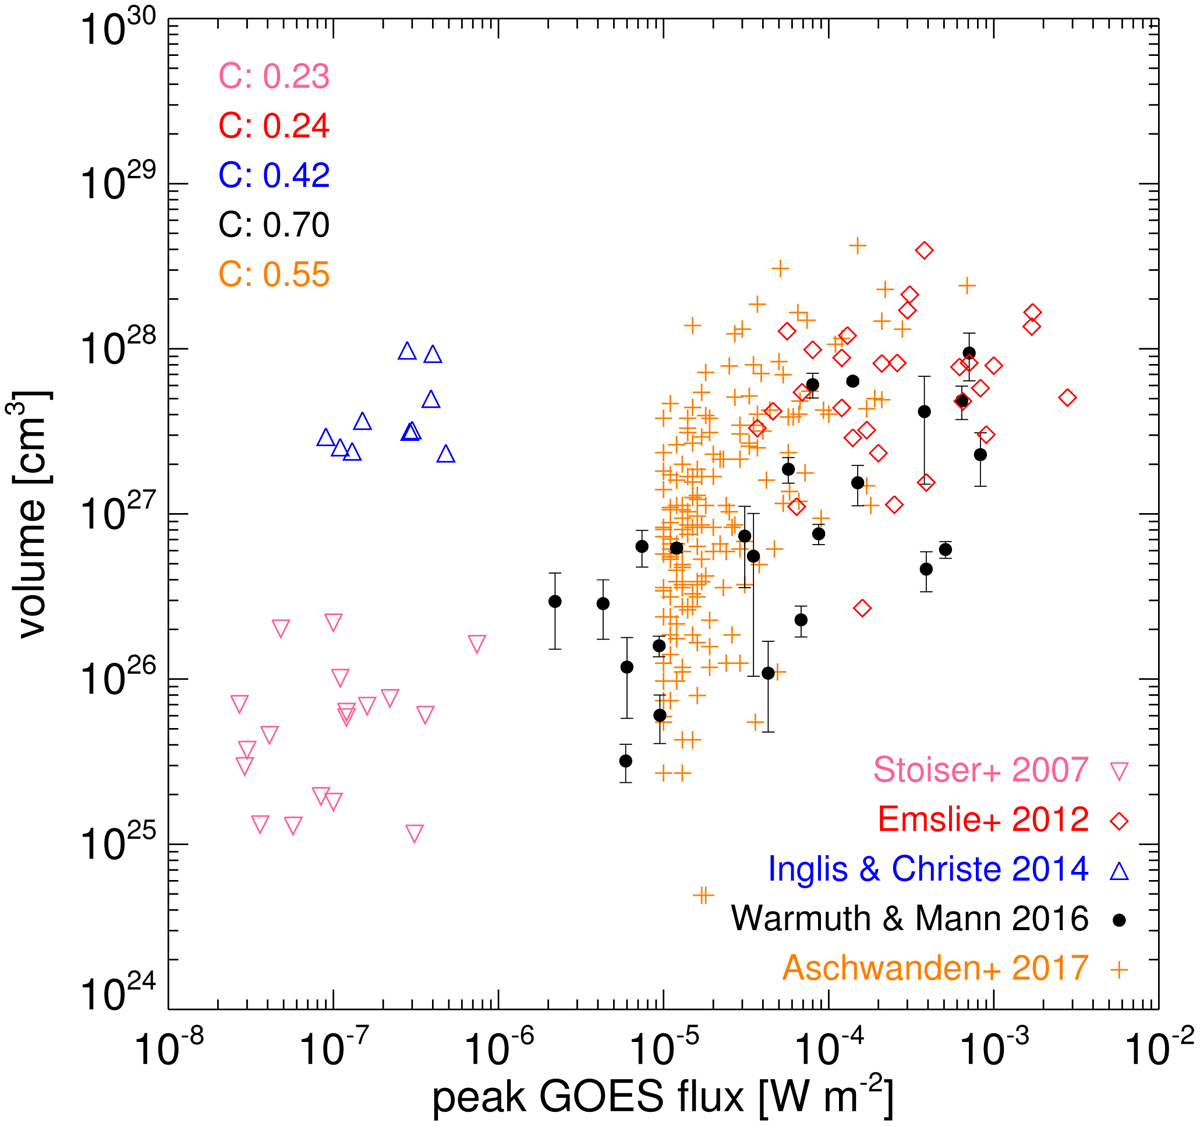
\includegraphics[width=0.45\textwidth,trim={0cm 0cm 0cm 0.02cm},clip]{goes_flux_vol.jpg}
    \caption{{\it GOES} peak thermal energy (left panel) and volume of the thermal plasma (right panel) as a function of the peak {\it GOES} flux for all the flares from five studies (figure credit: \cite{warmuth20}). The C values show the linear correlation coefficient for various studies.}
    \label{fig:goes-therm}
\end{figure}
%%%%%%%%%%%%%%%%%%%%%%%%%%%%%%%%%%%%%%%%%%%%%%%

The thermal energy estimated usually depends on the source volume, $U_{Th}\sim V$. Apart from S07 and A17, all other studies used {\it RHESSI} imaging to estimate the flare volume with a filling factor $f=1$. S07 determined the volume by employing a semicircular loop model, utilizing the cross-sectional area and loop length derived from the observed areas and separations of foot point brightening of 1600  {\AA} by {\it TRACE}. In contrast, A17 estimated the volume based on the flare area exceeding a certain threshold in the emission measure obtained from the spatial synthesis DEM method. Fig.~\ref{fig:goes-therm} right panel shows the volumes used for various studies to estimate the thermal energy as a function of the peak {\it GOES} flux. It is worth noting that the volume estimates from E12 and WM16 align closely, as do those from A+17, despite employing entirely different methodologies. In contrast, the micro flare volumes reported by IC14 are notably larger, ranging from one to two orders of magnitude beyond what would be anticipated based on the findings of the other four studies. Intriguingly, this discrepancy aligns with the additional volume required to account for the higher thermal energies observed in IC14. The uncertainty in detecting volume can be due to the CLEAN algorithm systematically overestimates the source size \citep{warmuth13a}. There has also been studies demonstrating that {\it RHESSI} has difficulties in resolving small sources \citep{dennis09,warmuth13b}, that would be applicable for small thermal sources in the micro flares. This illustrates the requirement for better volume estimation for better estimates of the thermal energy of flares.

We can conclude a few more puzzling questions from these studies as a whole:

%%%%%%%%%
\begin{itemize}
    \item The primary challenge in estimating the thermal energy of the hot plasma stems from determining the temperature distribution of the plasma using Differential Emission Measure (DEM), and the radiating plasma volume.
    \item The dissipation of energy from the hot plasma is substantial. Although there is widespread agreement regarding radiative losses across studies, the extent of conductive losses disagree significantly between the studies.
    \item The non-thermal energy in injected electrons is strongly dependent on the poorly constrained low-energy cutoff.
    \item The thermal and non-thermal energy partition changes with flare class. In smaller flares, there appears to be a deficiency of energetic electrons, whereas in larger flares, the injected non-thermal energy seems to sufficient in powering the thermal component. Does this signify the existence of an additional third heating source?
\end{itemize}
%%%%%%%%%


%% ################################################################# %%
\section{Motivation}\label{sec:mot}
%% ################################################################# %%

The main motivation of this thesis is to add understanding of effects of flares on the surrounding environment in lower and upper solar atmosphere, to answer some of the questions posed above. We have used imaging and spectroscopic observations from multiple space based observatories ({\it e.g.} AIA, HMI, IRIS, XRT, etc.). This research contributes to creating a perspective of flare energetics and its effect on the surrounding plasma environment from Chromosphere to Corona.

The solar flares are the strongest magnetic event in our solar system connecting various layers of the solar atmosphere ({\it e.g.} from Photosphere to Corona), coupled via mass and energy transport. While the Coronal manifestation of solar flares have been studied extensively with several instruments, there are only a few imaging and spectroscopic instruments observing the Photosphere to transition region. These include the {\it IRIS} \citep{iris}, AIA 1600, 1700, and 304  {\AA} \citep{aia} and some the filters of {\it Hinode}/SOT \citep{sot}. In addition to these, we also have had balloon experiment {\it SUNRISE} \citep{sunrise1,sunrise2}, which provided high resolution imaging of the transition regiopn, from the SuFI instrument \citep{sufi}.

This illustrates the necessity of more observatories operating at the transition region wavelengths for more comprehensive understanding about how the solar flares manifest and affect the dynamics and heating of the lower solar atmosphere. In this regard, {\suit} onboard Aditya-L1 will play a crucial role in probing the lower solar atmosphere. The various imaging channels of {\suit} would observe the manifestation of flares in transition region at various heights (NB3 $\implies$ \ion{Mg}{2} k 279.6 nm, NB4 $\implies$ \ion{Mg}{2} h 280.3 nm, NB8 $\implies$ \ion{Ca}{2} h 396.8 nm), further lower in the transition region (NB2 $\implies$ blue wing of Mg window, NB5 $\implies$ red wing of Mg window) and Sunspots and possible signature of umbral brightening due to flares at the Photosphere (NB6 300 nm and NB7 388 nm) in full disk. This would also allow us to probe the interaction of the flaring region, with other active regions on disk, giving us a comprehensive overview of the effect of solar flares and their manifestation in the lower solar atmosphere.

%% ################################################################# %%
\section{Outline of Thesis}\label{sec:outline}
%% ################################################################# %%

The work within this thesis spans across various layers of the solar atmosphere to understand how solar flare couples these layers. It is carried out partly, as various preparatory analysis for {\suit}, forward modelling {\suit} observations, designing the stellar calibration scheme for {\suit}, analysis of existing transition region observations in anticipation of {\suit} observations, analysis of coronal observations of solar flares, and analysis of first solar flare observations by {\suit}. Here we will briefly discuss the structure of the rest of the thesis:

%%%%%%%%%%%%%%%%%%%%%%%%%%%
\begin{itemize}
    \item In chapter \ref{c:chap2}, we review various space based missions available and used in this thesis. We also discuss various analysis techniques used in this thesis. We also motivate the importance of {\suit} and its main science goals. We also briefly discuss the specific questions regarding solar flares we can address with {\suit}.
    \item In chapter \ref{c:chap3}, we discussed some of the initial preparatory analysis we did for {\suit}, including the throughput model for {\suit}, how the filters mounted on {\suit} were chosen, the analysis of spacecraft jitter simulation and what effect it would have on the imaging. We also describe the stellar calibration scheme and the selection criteria for the standard star target. We use a sun as a star spectra to evaluate the calibration scheme with the aforementioned throughput model.
    \item In chapter \ref{c:chap4}, we discuss the forward modelling pipeline developed for {\suit}. We use MPS-Atlas simulation and {\it IRIS} observations, with measured transmission profiles of various optical components and the PSF to forward model {\suit} observations. We also discuss a preliminary version of the deconvolution algorithm that will be deployed in the data reduction pipeline.
    \item In chapter \ref{c:chap5}, we use existing {\it IRIS} observations of three solar flares to probe how the lower solar atmosphere is affected by the flares. The ratio of the \ion{Mg}{2} k and h lines, is a proxy for the optical depth of the surrounding plasma. Hence, we use the observations of \ion{Mg}{2} lines along HMI magnetic field measurements to investigate the effects of magnetic field, if any. \cite{kerr15} conducted a similar study and found signatures of localised heating in the line intensity ratio. We found, that the line intensity ratio shows a correlated increase and decrease with the flare light curve. We argue this to be signature of plasma flow associated with flare, and a change in density of the local environment. This acts as a prelude of what is achievable with {\suit}. We can use a similar method to give full disk context of optical depth, with respect to eruptive events.
    \item We address the issues raised in \S\ref{sol_flr_std_mod} regarding the uncertainties of volume estimation for flaring plasma and its effects on the thermal energy estimation in chapter \ref{c:chap6}. We use observations from {\it SDO}/AIA, {\it STEREO-A}/EUVI, {\it SO}/STIX, {\it GOES}/SUVI to estimate the thermal energy of two solar flares. We propose a new  using existing tools, to use observations from different vantages ({\it e.g.} AIA and EUVI from different angles) to accurately calculate the volume of the flare arcade and estimate the thermal energy. We show that the accurate estimate as a function of time can have effects on the accurate estimation of thermal energy and the partition between the thermal and non-thermal component.
\end{itemize}
%%%%%%%%%%%%%%%%%%%%%%%%%%%